\documentclass{lea}

%%
%% Setup
%%

\title{ENIGMA HALFpipe: Interactive, reproducible, and efficient analysis for resting-state and task-based fMRI data}

\author[1,\envelope]{\mbox{Lea Waller \orcid{0000-0002-3239-6957}}}
\author[1]{\mbox{Susanne Erk \orcid{0000-0003-0961-3543}}}
\author[2,3]{\mbox{Elena Pozzi \orcid{0000-0001-8360-5571}}}
\author[2,3]{\mbox{Yara J. Toenders \orcid{0000-0002-4117-1143}}}
\author[4]{\mbox{Courtney C. Haswell}}
\author[1]{\mbox{Marc Büttner \orcid{0000-0001-6940-6656}}}
\author[5]{\mbox{Paul M. Thompson \orcid{0000-0002-4720-8867}}}
\author[2,3]{\mbox{Lianne Schmaal \orcid{0000-0001-9822-048X}}}
\author[4\authfn{1}]{\mbox{Rajendra A. Morey \orcid{0000-0002-6517-6969}}}
\author[1\authfn{1}]{\mbox{Henrik Walter \orcid{0000-0002-9403-6121}}}
\author[1,6\authfn{1}]{\mbox{Ilya M. Veer \orcid{0000-0002-6733-3593}}}

\affil[1]{Charité Universitätsmedizin Berlin, corporate member of Freie Universität Berlin and Humboldt-Universität zu Berlin, Department of Psychiatry and Psychotherapy CCM, Berlin, Germany}
\affil[2]{Centre for Youth Mental Health, University of Melbourne, Melbourne, Australia}
\affil[3]{Orygen, Parkville, Australia}
\affil[4]{Duke University School of Medicine, Durham, NC, USA}
\affil[5]{Imaging Genetics Center, Mark and Mary Stevens Institute for Neuroimaging and Informatics, Keck School of Medicine, University of Southern California, Los Angeles, CA, USA}
\affil[6]{Donders Institute for Brain, Cognition and Behaviour, Nijmegen, the Netherlands; Radboud University Medical Center, Nijmegen, the Netherlands}
\affil[\envelope]{Correspondence should be addressed to \href{mailto:lea@fmri.science}{lea@fmri.science}}

\contrib[\authfn{1}]{These authors contributed equally to this work}

\fancyhead[L]{\sffamily Waller et al.}
\fancyhead[R]{\sffamily ENIGMA HALFpipe | {\fontseries{mb}\selectfont\color{leaPurple}\thepage}}

\fancyfoot[C]{}
%\fancyfoot[R]{\sffamily%
%\href{https://github.com/HALFpipe/HALFpipe}{\color{leaPurple}{https://github.com/HALFpipe/HALFpipe}}}

% hyphenation exceptions
\hyphenation{fMRIPrep}

\addbibresource{./bib/ilya.bib}
\addbibresource{./bib/lea.bib}


%%
%% Article
%%

\begin{document}

\maketitle

\begin{abstract}

The reproducibility crisis in neuroimaging has led to an increased
demand for standardized data processing workflows. Within the ENIGMA
consortium, we developed \soft{HALFpipe} (\myuline{H}armonized 
\myuline{A}na\myuline{L}\contour{white}{ysis} of \myuline{F}unctional MRI 
\myuline{pipe}line), an open-source, containerized, user-friendly tool that
facilitates reproducible analysis of task-based and resting-state fMRI
data through uniform application of preprocessing, quality assessment,
single-subject feature extraction, and group-level statistics. It
provides state-of-the-art preprocessing using \soft{fMRIPrep} without the
requirement for input data in Brain Imaging Data Structure (BIDS)
format. \soft{HALFpipe} extends the functionality of \soft{fMRIPrep} with 
additional preprocessing steps, which include spatial smoothing, grand 
mean scaling, temporal filtering, and confound regression. \soft{HALFpipe}
generates an interactive quality assessment (QA) webpage to assess the quality of
key preprocessing outputs and raw data in general. \soft{HALFpipe} features
myriad post-processing functions at the individual subject level,
including calculation of task-based activation, seed-based connectivity,
network-template (or dual) regression, atlas-based functional
connectivity matrices, regional homogeneity (ReHo), and fractional
amplitude of low frequency fluctuations (fALFF), offering support to
evaluate a combinatorial number of features or preprocessing settings in
one run. Finally, flexible factorial models can be defined for
mixed-effects regression analysis at the group level, including multiple
comparison correction. Here, we introduce the theoretical framework in
which \soft{HALFpipe} was developed, and present an overview of the main
functions of the pipeline. \soft{HALFpipe} offers the scientific community a
major advance toward addressing the reproducibility crisis in
neuroimaging, providing a workflow that encompasses preprocessing,
post-processing, and QA of fMRI data, while broadening core principles
of data analysis for producing reproducible results. Instructions and 
code can be found at \url{https://github.com/HALFpipe/HALFpipe}.

\end{abstract}

\section{Introduction}

The application of neuroimaging, in particular functional MRI (fMRI), has
led to an explosion in knowledge about brain functions implicated in a
range of human behaviors, cognitive processes, and emotions. Such research
has been spurred by rapid advances in computationally intensive software
required to perform complex algorithmic processing and statistical modeling
of fMRI data. The resulting proliferation of software tools designed to
fulfill various analytic functions has produced a large array of options
for carrying out any given type of processing. Since the fMRI signal
indirectly captures the neural processes of interest, a series of
computational operations on fMRI data, referred to as the \term{analysis
pipeline}, are necessary to arrive at interpretable results. In practice,
each step is flexible and subject to a number of choices by the researcher,
termed \term{analytic flexibility} \citep{10.1038/nrn.2016.167}. The steps
in the analysis pipeline may be reordered, run with different parameters,
or may be completely omitted in some cases. Understandably, users expect
different tools performing the same function to generate (near) identical
results when supplied with given input data. However, the multiplicity of
tools has had the unintended consequence of generating inconsistent results
from studies designed to answer the same research question, sometimes even
when the same data is used as the starting point
\citep{10.1038/s41586-020-2314-9}. Thus, \term{analytic flexibility}
combined with the number of analysis steps, as well as the possible
parameters for running each analysis step, has led to a vast multiplicity
of methodologic variants and an equal number of possible results. This
situation has contributed in part to what is widely hailed as a
\term{crisis of reproducibility,} which now plagues the neuroimaging field
\citep{10.1038/sdata.2016.44,10.1038/nrn.2016.167}.

One solution to improving reproducibility is to constrain the parameter
space by limiting choices to default parameters established from
empirically-derived best-practices \citep{10.1016/j.cels.2018.03.014}. For
instance, established pipelines such as \soft{fMRIPrep}
\citep{10.1038/s41592-018-0235-4} and \soft{C-PAC}
\citep{craddock_towards_2013} have automated many of these choices. An
alternative approach is to run multiple analyses separately on the same
input data with the same or different pipelines, but with different
parameter selections for each analysis, and then compare the results. This
second approach, termed \term{multiverse analysis}
\citep{10.1177/1745691616658637}, has the advantage that results from
multiple analyses may be compared and alternate solutions may be presented
in published reports to promote increased transparency. However,
\term{multiverse analysis} has the disadvantage that it may ultimately not
be possible to determine the optimal or even the correct solution, as true
effects in non-simulated fMRI data are often unknown.

The reproducibility crisis has led to an increased demand for standardized
workflows to conduct both the preprocessing and postprocessing stages of
fMRI analysis. The recent introduction and widespread adoption of
standardized pipelines for fMRI data preprocessing has provided the
research community with much-needed high-quality tools that have improved
reproducibility \citep{thompson_big_2020}. The four ingredients that are
essential to data analysis and reproducible results are: (1) data and
metadata availability, (2) code usage and transparency, (3) software
installability, and (4) re-creation of the runtime environment. Relative to
other processing pipelines, \soft{fMRIPrep}
\citep{10.1038/s41592-018-0235-4} has grown in popularity due to its
adoption of best practices, open-source availability, favorable user
experience, and \term{glass-box} principles of transparency
\citep{10.1146/annurev-biodatasci-072018-021237}. However, \soft{fMRIPrep}
is limited to the so-called preprocessing steps of fMRI data analysis,
whilst variability in parameter selection for subsequent post-processing
analysis steps (e.g., data cleaning, feature extraction, model
specification) may compromise reproducibility.

The ENIGMA consortium has addressed the reproducibility crisis by pooling
observational study data from structural and diffusion imaging (and more
recently EEG and MEG), and by developing standardized pipelines, data
harmonization methodology, and quality control protocols
\citep{thompson_enigma_2020}. These workflows have successfully analyzed
structural and diffusion MRI data aggregated from large numbers of small-
and medium-sized cohorts to accumulate sufficient power to yield robust
results on a wide range of neuropsychiatric conditions
\citep[e.g.][]{10.1038/s41398-020-0842-6,van_den_heuvel_overview_2020,10.1002/hbm.25029}.
However, until now the ENIGMA consortium has lacked the ability to reliably
conduct consortium-wide analyses on fMRI data. More recently, however, the
ENIGMA task-based \citep{veer_enigma_2019} and resting-state fMRI
\citep{10.1007/s11682-018-9941-x} working groups have spurred initiatives
to bring the ENIGMA framework to the functional domain.

To support these initiatives within ENIGMA, we developed a standardized
workflow that encompasses the essential elements of task-based and
resting-state fMRI analyses from raw data to group-level statistics, builds
on the progress and contributions of \soft{fMRIPrep} developers, and
extends its functionality beyond preprocessing steps to include additional
preprocessing, post-processing, and interactive tools for quality
assessment. These extended features include: automatic and reliable
conversion of fMRI data to BIDS format, spatial smoothing, temporal
filtering, extended confounds regression, calculation of task-based
activations, and resting-state feature extraction, including seed-based
functional connectivity, network-template (dual) regression, atlas-based
functional connectivity matrices, regional homogeneity (ReHo) analysis, and
fractional amplitude of low frequency fluctuations (fALFF). Although each
of these post-processing functions is available in other software packages
and a few pipelines have incorporated a subset of these features,
\soft{HALFpipe} combines all these post-processing tools from open-source
neuroimaging packages with the preprocessing steps performed by
\soft{fMRIPrep} (see Table~\ref{table:comparison}). Furthermore, although
\soft{HALFpipe} provides recommended settings for each of the processing
steps (see Table~\ref{table:settings}), it allows users to run any combinatorial
number of these processing settings, thereby offering a streamlined
infrastructure for pursuing multiverse analyses. Similar to other
processing pipelines, \soft{HALFpipe} is available as a containerized
image, thereby offering full control over the computational environment.
In this article, we provide a detailed description of \soft{HALFpipe}. 
First we explain the software architecture and implementation, followed by
a walkthrough of the procedure for running the software, and finally a 
discussion of the potential applications of the pipeline.

\begin{tablebox}[label={table:comparison}]{Comparison to other neuroimaging pipelines}

\begingroup%
\newcolumntype{L}{>{\raggedright\arraybackslash}X}%
\newcolumntype{C}{>{\centering\arraybackslash}X}%
% \newcommand{\conditionalformat}[1]{% 
%     \IfStrEqCase{#1}{Yes}{% 
%         \cellcolor{leaLightGreen}#1
%     }{No}{%
%         \cellcolor{leaLightYellow}#1
%     }[%
%         #1
%     ]%
% }
% \newcolumntype{K}{>{\collectcell\usermacro}X{\endcollectcell}}%
\renewcommand\tabularxcolumn[1]{m{#1}}%
\renewcommand{\arraystretch}{1.3}%
\begin{tabularx}{\textwidth}{@{} | L | L | 
C | C | C | C | C | C | @{}} 
\hhline{~|~|-|-|-|-|-|-|}
\multicolumn{2}{c|}{} &%
\textbf{HALFpipe} &%
\textbf{C-PAC} &%
\textbf{fMRIPrep MRIQC FitLins} &%
\textbf{CONN toolbox} &%
\textbf{XCP Engine} &%
\textbf{DPARSF DPABI} \\
\hhline{-|-|-|-|-|-|-|-|}
\multirow{2}{*}[-1.3em]{\parbox[c][][c]{2cm}{\raggedright{Quality assessment}}} &%
Quality metrics &%
\cellcolor{leaLightGreen}Yes &% 
\cellcolor{leaLightGreen}Yes &% 
\cellcolor{leaLightGreen}Yes &% 
\cellcolor{leaLightGreen}Yes &% 
\cellcolor{leaLightGreen}Yes &%
\cellcolor{leaLightGreen}Yes \\
\hhline{~|-|-|-|-|-|-|-|}
&%
Visual quality assessment &%
\cellcolor{leaLightGreen}Yes &%
\cellcolor{leaLightGreen}Yes &%
\cellcolor{leaLightGreen}Yes &%
\cellcolor{leaLightGreen}Yes &%
\cellcolor{leaLightGreen}Yes &%
\cellcolor{leaLightGreen}Yes \\
\hhline{-|-|-|-|-|-|-|-|}
\multirow{7}{*}[-3.3em]{Features} &% 
Task-based activation &%
\cellcolor{leaLightGreen}Yes &%
\cellcolor{leaLightYellow}No &%
\cellcolor{leaLightGreen}Yes &%
\cellcolor{leaLightYellow}No* &%
\cellcolor{leaLightGreen}Yes &%
\cellcolor{leaLightYellow}No \\
\hhline{~|-|-|-|-|-|-|-|}
& Seed-based connectivity &%
\cellcolor{leaLightGreen}Yes &%
\cellcolor{leaLightGreen}Yes &%
\cellcolor{leaLightYellow}No &%
\cellcolor{leaLightGreen}Yes &%
\cellcolor{leaLightGreen}Yes &%
\cellcolor{leaLightGreen}Yes \\
\hhline{~|-|-|-|-|-|-|-|}
& Dual regression &%
\cellcolor{leaLightGreen}Yes &%
\cellcolor{leaLightGreen}Yes &%
\cellcolor{leaLightYellow}No &%
\cellcolor{leaLightGreen}Yes &%
\cellcolor{leaLightYellow}No &%
\cellcolor{leaLightGreen}Yes \\
\hhline{~|-|-|-|-|-|-|-|}
& Atlas-based connectivity matrix &%
\cellcolor{leaLightGreen}Yes &%
\cellcolor{leaLightGreen}Yes &%
\cellcolor{leaLightYellow}No &%
\cellcolor{leaLightGreen}Yes &%
\cellcolor{leaLightGreen}Yes &%
\cellcolor{leaLightGreen}Yes \\
\hhline{~|-|-|-|-|-|-|-|}
& ReHo &%
\cellcolor{leaLightGreen}Yes &%
\cellcolor{leaLightGreen}Yes &%
\cellcolor{leaLightYellow}No &%
\cellcolor{leaLightGreen}Yes** &%
\cellcolor{leaLightGreen}Yes &%
\cellcolor{leaLightGreen}Yes \\
\hhline{~|-|-|-|-|-|-|-|}
& fALFF &%
\cellcolor{leaLightGreen}Yes &%
\cellcolor{leaLightGreen}Yes &%
\cellcolor{leaLightYellow}No &%
\cellcolor{leaLightGreen}Yes &%
\cellcolor{leaLightGreen}Yes &%
\cellcolor{leaLightGreen}Yes \\
\hhline{~|-|-|-|-|-|-|-|}
& Group statistics &%
\cellcolor{leaLightGreen}Yes &%
\cellcolor{leaLightGreen}Yes &%
\cellcolor{leaLightGreen}Yes &%
\cellcolor{leaLightGreen}Yes &%
\cellcolor{leaLightYellow}No &%
\cellcolor{leaLightGreen}Yes \\
\hhline{-|-|-|-|-|-|-|-|}
\end{tabularx}\par
\vspace*{2mm}
Note: * task-based connectivity is supported; ** as implemented with LCOR (Local Correlation).
\endgroup

\end{tablebox}



\section{Methods}

The \soft{HALFpipe} software is containerized, similar to \soft{fMRIPrep}
or \soft{C-PAC}. This means that it comes bundled with all other software
that is needed for it to run, such as \soft{fMRIPrep}
\citep{10.1038/s41592-018-0235-4}, MRIQC
\citep{10.1371/journal.pone.0184661}, FSL
\citep{10.1016/j.neuroimage.2011.09.015}, ANTs
\citep{10.1016/j.neuroimage.2010.09.025}, FreeSurfer
\citep{10.1073/pnas.200033797}, and AFNI
\citep{10.1006/cbmr.1996.0014,10.1002/(sici)1099-1492(199706/08)10:4/5<171::aid-nbm453>3.0.co;2-l}.
As such, all users of one version of \soft{HALFpipe} will be using the
exact same versions of these tools, because they come with the container.
Thus, the containerization of \soft{HALFpipe} software aids reproducibility
across different researchers and computing environments. We have provided
the \soft{HALFpipe} application in a Singularity container and a Docker
container. Singularity or Docker, which are both freely available, must be
installed prior to downloading the containerized \soft{HALFpipe}
application. Both Docker and Singularity perform so-called
operating-system-level virtualization, but are more efficient and require
less resources than virtual machines. Running Docker containers on a Linux
or macOS operating system requires administrator privileges. Singularity is
typically run on a Linux operating system, which may be used without
administrator privileges.

Besides containers, our \soft{HALFpipe} development team adopted other
software engineering best practices, which promoted faster development and
reduced code errors. These industry best-practices, which have found their
way into research applications \citep{das_programming_2018}, involve
writing code that is easy to read (albeit generally harder to write), the
breakdown of complex systems into several simpler subsystems, dedicated
effort toward thoughtful code design before implementation, and performing
continuous integration via unit tests \citep{beckkent2000epe:}. The
\soft{HALFpipe} development team applied these practices whenever possible.

\soft{HALFpipe} is being developed as an open-source project and is
accepting contributions that offer new features, enhance functionality, or
improve efficiency. All changes will be reviewed manually. Additionally,
before inclusion in the source tree, changes will undergo automated (unit)
testing, which includes running an entire analysis for one subject of the
OpenNeuro dataset ds000108 \citep{10.1016/j.neuron.2008.09.006}. This way,
unexpected side effects and bugs can be caught and corrected before causing
problems for users.

\subsection{Databases}

To automatically construct a neuroimaging processing workflow, the program
needs to be able to fulfill queries such as \pseudocode{retrieve the
structural image for subject x}. Many programs implement such queries using
a database system. 

For example, the Python implementation of the BIDS
standard, called \soft{PyBIDS}, uses an SQL database on the back-end. Each
file of a BIDS dataset is assigned a number of tags in the database, such
as \code{subject}, \code{task}, or \code{session} to facilitate executing
queries on these tags. The PyBIDS equivalent of the example above would be
\code{layout.get(datatype='anat', sub='x')}. The database approach adds a
layer of complexity, because the database must be defined and populated and
code must be written to interface with the database. For \soft{HALFpipe},
we chose to construct indices and query functions based on native Python
data types.

A further challenge is generating database queries that flexibly interface
with the logic of neuroimaging and processing pipelines, which is relevant
in the context of missing data. \soft{HALFpipe} always tries to execute the
best possible processing pipeline based on the data that is available. For
example, a field map may have been routinely acquired before each
functional scan in a particular dataset. If one of these field maps is
missing, \soft{HALFpipe} flexibly assigns another field map, for example
one belonging to the preceding functional scan. However, \soft{HALFpipe}
will not use a field map from another scan session, as field
inhomogeneities are likely to have changed. Finally, \soft{HALFpipe} does
not fail if a field map is missing, but simply omits the distortion
correction step for that subject. Other examples include the ability of
\soft{HALFpipe} to match structural to functional images, and match task
events to a functional scan. This strategy is used throughout the
construction of processing workflows.

\subsection{Metadata}

Processing of neuroimaging data requires access to relevant metadata, such
as temporal resolution, spatial resolution, and many others. Some elements
of metadata, such as echo time (TE), are represented differently depending
on scanner manufacturer and DICOM conversion software. The method for
reading various types of data has been harmonized in \soft{HALFpipe} using
the following three methods.

First, metadata can be stored in BIDS format. This means that a JavaScript
Object Notation (JSON) file accompanies each image file, which contains the
necessary metadata. BIDS calls this file the \term{sidecar}, and common
tools such as \soft{heudiconv} \citep{yaroslav_halchenko_2018_1306159} or
\soft{dcm2niix} \citep{10.1016/j.jneumeth.2016.03.001} generate these files
automatically. If these files are present, \soft{HALFpipe} will detect and
use them. Second, instead of sidecar files, some software tools store image
metadata in the NIfTI header. The NIfTI format defines fields that can fit
metadata, but depending on how the image file was created, these metadata
may be missing. Some conversion programs also place the metadata in the
description field in free text format. This description can also be parsed
and read automatically. Third, information may be incorrectly represented
due to user error, incompatible units of measurement, or archaic technical
considerations. In such cases, \soft{HALFpipe} provides a mechanism to
override the incorrect values. For every metadata field, the user interface
will prompt the user to confirm that metadata values have been read or
inferred correctly. The user can choose to manually enter the correct
values.

\subsection{Interfaces}

\soft{HALFpipe} consists of different modules that need to pass data
between each other, such as file pathnames and the results of quality
assessment procedures. Developing an application as large and complex as
\soft{HALFpipe} requires establishing predictable interfaces, which
prescribe data formats for communication within the application. An
advantage of this approach is that knowledgeable users can write their own
code to interface with \soft{HALFpipe}.

\soft{HALFpipe} uses the Python module \soft{marshmallow} to implement
interfaces, called schemas in the module's nomenclature. All schemas are
defined in the \soft{HALFpipe} code. When the user first starts the
application, the user interface is displayed by \soft{HALFpipe}. It asks
the user a series of questions about the data set and the analysis plan,
and stores the inputs in a configuration file called \filename{spec.json}. The
configuration file has a predictable syntax and can be easily scripted or
modified, which enables collaborative studies to harmonize analysis plans.

\subsection{Workflow engine}

To obtain reproducible results, a core requirement for \soft{HALFpipe} was
reproducible execution of the processing pipeline. As the ENIGMA consortium
requires fMRI analysis of large datasets with several thousand samples,
\soft{HALFpipe} was designed to parallelize processing on multiple
computers or processor cores. Both of these specifications were achieved by
implementation in \soft{Nipype}, \term{NeuroImaging in Python: Pipelines
and Interfaces} \citep{10.3389/fninf.2011.00013}. \soft{Nipype} is a
workflow engine for neuroimaging that constructs an acyclic directed graph,
in which nodes represent processing commands that need to be executed (the
steps of the pipeline), while the edges represent inputs and outputs being
passed between nodes (images or text files). In this formalization of a
neuroimaging pipeline as a graph, the fastest order for execution across
multiple processor cores can be determined.

The workflow graphs are modular and scalable, which means they can be
nested and extended. \soft{HALFpipe} uses the workflows defined by
\soft{fMRIPrep} and then connects their outputs to additional workflows.
\soft{fMRIPrep} itself is modular and divided into multiple workflows:
\soft{sMRIPrep} \citep{esteban_oscar_2021_4593442}, \soft{SDCFlows}, and
\soft{NiWorkflows}. The workflow graph facilitates saving and verifying
intermediate results, and supports the user's ability to stop and later
restart processing. \soft{HALFpipe} also uses the graphs to determine which
intermediate results files are not needed by subsequent commands by using a
tracing garbage collection algorithm \citep{10.1145/359642.359655}. As
such, intermediate files do not accumulate on the storage device. This
feature is implemented as a plugin to \soft{Nipype}.

\soft{Nipype} forms the basis of \soft{fMRIPrep} and \soft{C-PAC}, which
are widely used in the neuroimaging community. However, it has several
limitations that are relevant in the context of \soft{HALFpipe}.
\soft{HALFpipe} is able to calculate features and statistical maps with
different variations of preprocessing settings. To do this efficiently,
intermediate results need to be re-used whenever possible. An improved
second version of \soft{Nipype} is currently being developed, called
\soft{Pydra} \citep{pydra-proc-scipy-2020}, which will be able to
automatically detect repetitive processing commands, and automatically
re-use outputs. Presently, until \soft{Pydra} becomes available,
\soft{HALFpipe} calculates a four-letter hash code that uniquely identifies
each preprocessing step. Before constructing a new preprocessing command,
\soft{HALFpipe} checks whether its hash has already been added to the
graph. If present, the existing command is re-used.

A key requirement of \soft{HALFpipe} was robust and flexible handling of
missing data. For instance a missing functional scan or statistical map
does not cause \soft{HALFpipe} to fail. Additionally, \soft{HALFpipe}
defines inclusion and exclusion criteria for scans, such as the maximum
allowed motion (mean framewise displacement) or a minimum brain coverage
when extracting a brain region's average signal. Finally, depending on the
data set, statistical maps may need to be aggregated across runs or
sessions within single subjects before a group-level model can be run. This
means that the static graph has to be modified dynamically to adapt to the
results of processing. \soft{HALFpipe} solves this problem by defining a
data structure that not only contains the file names of statistical maps,
but also the tags and metadata that can be used to adjust processing on the
fly. For example, using this data structure, design matrices can be
constructed for group models based on the actual subjects that have
statistical maps available.

\subsection{Running on a high-performance cluster}

\soft{HALFpipe} provides a simple way to run on a high-performance compute
cluster. For each subject, preprocessing and feature extraction takes 6 to
10 hours on a single processor core. Most jobs take about 8 GB to 20 GB of
RAM, depending on size of the data. Assuming each subject is assigned to a
unique job, we recommend requesting 24 GB of RAM for each job. The most
memory-intensive steps of processing are spatial registration and
resampling, and running \soft{FSL MELODIC} for independent component
analysis (ICA) as part of \soft{ICA-AROMA}
\citep{10.1016/j.neuroimage.2015.02.064}. For large datasets, parallel
processing of subjects is highly desirable to reduce the total computation
time.

Deploying \soft{Nipype} to perform computations on multiple nodes, such as
on a high performance cluster (HPC) is particularly challenging. By
default, \soft{Nipype} submits a separate job to the cluster queue for each
processing command (graph node) regardless of the amount of time required
to execute the command. A watcher process running on the head node collects
outputs from completed commands and submits the next processing command.
This process can be inefficient on some HPCs because computational
resources need to be allocated and deallocated continually. We implemented
a more efficient approach for \soft{HALFpipe} that partitions the
processing graph into many independent subgraphs, which the user may submit
as separate jobs. The smallest granularity available is one subgraph per
subject that is invoked with the command line flag \code{--subject-chunks}.
A \soft{Nipype} workflow is created and validated for all subjects before
the pipeline starts running. In a cluster setting, the most efficient
resource utilization is to submit each subject as a separate job and to run
each job on two CPU cores.

\subsection{Data denoising}\label{sec:denoising}

\soft{HALFpipe} and \soft{fMRIPrep} are modular preprocessing pipelines,
meaning that they utilize a series of tools from various software
libraries. Most have been adopted as standard practice by the community for
many years. Thus, the reasons motivating specific algorithmic choices may
not be readily apparent to users, but need to be considered when designing
tools such as \soft{HALFpipe}. Here we articulate the design considerations
in our selection of tools.

\soft{HALFpipe} performs all denoising in a predefined order after
resampling the fMRI data to standard space using \soft{fMRIPrep}.
\soft{HALFpipe} defines standard space as the \term{MNI152NLin2009cAsym}
template, which is the most current and detailed template available
\citep{horn_blog}.

\soft{fMRIPrep} not only outputs a preprocessed image in standard space,
but also a spreadsheet with nuisance (or confound) time series. These
include (derivatives of) motion parameters (squared), aCompCor components
\citep{10.1016/j.neuroimage.2007.04.042}, white matter signal, CSF signal,
and global signal. A key consideration is that including these time series
as nuisance regressors may re-introduce variance that was already removed
in previous processing steps \citep{10.1016/j.neuroimage.2013.05.116}. An
example of this phenomenon may be regressing out motion parameters after
removing low-frequency drift via temporal filtering. In practice, this
means setting up a regression model for each voxel, where the temporally
filtered time series of a voxel is the dependent variable and the
regressors are the motion parameters. The regression model will calculate a
regression weight for each motion regressor, so that the total model
explains the maximum amount of variance (under assumption of normality).
After multiplying the motion parameters with these weights, they are summed
to yield one time series containing the motion-related noise. This time
series is subtracted from the temporally filtered voxel time series to
yield the result of the procedure, the denoised time series (i.e., the
regression residuals). However, if the motion parameters happen to contain
any low-frequency drift, then their weighted sum likely will as well. It
follows that subtracting a time series with temporal drift from the
temporally filtered voxel data will introduce temporal drift again,
independent of whether a temporal filter was applied before. In
\soft{HALFpipe}, any filter or transformation applied to the voxel time
series is also applied to the nuisance time series. This way, previously
removed variance is not re-introduced accidentally, because it has been
removed from both sides of the regression equation. In \soft{HALFpipe},
denoising is implemented as follows:

\begin{enumerate}[leftmargin=*]

\item

\soft{ICA-AROMA} noise component classification
\citep{10.1016/j.neuroimage.2015.02.064} relies on reference masks defined
in \term{MNI152NLin6Asym} space, which is different from the standard space
template used by \soft{fMRIPrep}. To solve this issue, \soft{fMRIPrep} will
estimate a second normalization to this template, apply it to the fMRI
image in native space, and run \soft{ICA-AROMA} on the resulting image
\citep{10.1101/2021.02.10.430678}. This approach effectively doubles the
processor time spent on spatial normalization, and may require manually
checking both spatial registrations. To avoid this considerable effort,
\soft{HALFpipe} resamples the image to \term{MNI152NLin6Asym} space using
an existing transformation/warp field between the two spaces
\citep{horn_transform}. Specifically, this predefined warp field is
concatenated with the subject's warp to \term{MNI152NLin2009cAsym} space,
with which resampling is performed with \soft{fMRIPrep}'s
\code{bold\_std\_trans\_wf} workflow. Finally, \soft{ICA-AROMA} is run on the
resulting fMRI image in \term{MNI152NLin6Asym} space using
\soft{fMRIPrep}'s \term{ica\_aroma\_wf} workflow, which also includes spatial
smoothing fixed to a 6 mm FWHM smoothing kernel
\citep{10.1016/j.neuroimage.2015.02.064}. \soft{ICA-AROMA} generates a set
of component time series and a binary classification of these components as
either signal or noise.

\item

\soft{HALFpipe} implements spatial smoothing using \soft{AFNI}'s
\soft{3dBlurInMask} \citep{10.1006/cbmr.1996.0014}. Each voxel's signal is
averaged with the signal of its neighboring voxels, weighted by an
isotropic gaussian kernel. At the edges of the brain, this kernel may
include non-brain voxels, so smoothing is constrained to only happen within
the brain mask. This is equivalent to the procedure in the \term{Minimal
Preprocessing Pipelines for the Human Connectome Project}
\citep{10.1016/j.neuroimage.2013.04.127}.

\item\label{itm:grandmean}

Grand mean scaling sets the image mean, defined as the within-scan mean
across all voxels and time points, to a predefined value. The grand mean is
closely related to scanner parameters such as amplifier gain but not to
neural mechanisms \citep{10.1006/nimg.2002.1226}. Adjusting the grand mean
via scaling makes analysis results more interpretable and comparable across
subjects, sessions, and sites. The scaling factor is calculated based on
the masked functional image, and applied to both the fMRI data and the
nuisance time series extracted by \soft{fMRIPrep}.

\item\label{itm:aroma}

The previously estimated \soft{ICA-AROMA} noise components are removed from
the smoothed and grand-mean-scaled fMRI data. This is done in a
non-aggressive way to minimize removing variance that is shared between
signal and noise components. ICA-AROMA implements this step using the FSL
command \soft{fsl\_regfilt}, which calculates an ordinary least squares
regression for each voxel, where the design matrix includes both the signal
and the noise components as regressors. This means that the resulting
regression weights reflect the unique variance of the noise components (and
not the shared variance with signal components). Then, the noise component
regressors are multiplied by their regression weights and added together to
yield one time series of all the noise. Subtracting the noise from the
voxel time series yields a denoised time series (the regression residuals);
this step is done using a re-implementation of \soft{fsl\_regfilt} in
\soft{Numpy} \citep{10.1038/s41586-020-2649-2}. The same procedure is
applied to the nuisance time series from step~\ref{itm:grandmean}.

\item\label{itm:tempfilt}

Temporal filtering can be used to remove low-frequency drift via a
high-pass filter, high-frequency noise via a low-pass filter, or both at
the same time using a band-pass filter. \soft{HALFpipe} implements two
approaches to temporal filtering, a frequency-based approach
\citep{10.1155/2013/935154} and a Gaussian-weighted approach
\citep{10.1006/nimg.2000.0628}. The frequency-based temporal filter is very
exact in selecting frequencies to be kept or removed, and is commonly used
to calculate fractional Amplitude of Low Frequency Fluctuations (fALFF) and
Regional Homogeneity (ReHo). The Gaussian-weighted temporal filter is the
default used by \soft{FSL Feat} \citep{10.1016/j.neuroimage.2011.09.015}
and may have fewer edge effects at the start and end of the time series.
However, its spectrum also has a more gradual roll-off, meaning that it
will be less aggressive in removing frequencies close to the chosen cutoff
value. Temporal filtering is applied to both the fMRI data and nuisance
time series from step~\ref{itm:aroma}.

\item

Nuisance time series from step~\ref{itm:tempfilt} are removed using the
regression residualization procedure described above from both the fMRI
data and the nuisance time series.

\end{enumerate}

\soft{HALFpipe} suggests default settings for each of these steps, which
are outlined in \autoref{table:settings}. Note that some are selected based on
best-practices in the field (i.e., band-pass temporal filter for ALFF and
ReHo), whereas most default settings can be adjusted by the user.

\subsection{Quality assessment}\label{sec:qamethods}

Assessing the quality of data and preprocessing is a laborious undertaking
and often done manually. Efforts to automate this process, either through
predefined thresholds of image quality features
\citep{10.1016/j.neuroimage.2017.10.034} or machine learning
\citep{10.1371/journal.pone.0184661} are not yet ready to replace the eyes
of a trained researcher checking the data. However, various approaches make
this process easier. First, rather than viewing three-dimensional
neuroimaging files directly, generating and viewing reports containing
two-dimensional images offers a significant time savings. Second, tools
such as \soft{slicesdir} (in \soft{FSL}), \soft{fMRIPrep}, and \soft{MRIQC}
generate HTML files that contain multiple report images and can be explored
in a web browser. \soft{MRIQC} also provides an interactive widget to rate
the quality of each image \citep{10.1038/s41597-019-0035-4}.

In \soft{HALFpipe}, we use a fixed set of processing steps for quality
assessment. While \soft{slicesdir} allows the researcher to easily compare
the same image type across different subjects, it cannot be used to
generate reports for all types of images. By contrast,
\soft{fMRIPrep}/\soft{MRIQC} HTML files have a broad range of information
and quality report images included, but one HTML file is always specific to
one subject. As such, examining multiple processing steps in many subjects
can be cumbersome. To overcome these issues, \soft{HALFpipe} provides an
interactive web app that is contained in a single HTML file. The app
dynamically loads reports with images, and can handle datasets up to
thousands of images without a performance penalty. The images can be sorted
both by subject, as is done by \soft{fMRIPrep}/\soft{MRIQC}, or by image
type, as is done in \soft{slicesdir}. Each image can be rated as either
good, uncertain, or bad. Predefined logic automatically converts these
ratings into inclusion/exclusion decisions for \soft{HALFpipe}'s group
statistics. In addition, tagging images as uncertain enables users to
efficiently retrieve and discuss these with a colleague or collaborator,
after which a definitive decision on image quality can be made.

Images can be zoomed by clicking them. For faster operation by advanced
users, rating and navigation are accessible not just via user interface
buttons, but also via keyboard shortcuts based on the WASD keys. Pressing
the A goes back one image and D goes ahead, whereas W, S and X rate an
image as good, uncertain or bad, respectively. The web app offers an
overview chart that indicates subjects preprocessed successfully and
subjects with errors, a chart with quality ratings, and box plots
reflecting the sample distributions for motion, noise components, and
temporal signal-to-noise ratio (tSNR). All three are implemented so that
users can hover over chart elements with their cursor to view
meta-information, such as the subject identifier, and click to navigate to
the associated report images. The HTML file is built as a frameworkless web
app using TypeScript. Source code is available at
\url{https://github.com/HALFpipe/QualityCheck}.

\soft{HALFpipe} shows two report images for each subject on
structural/anatomical processing and four additional images for each type
of functional scan. Detailed explanations may be found in the quality
assessment manual at
\url{https://github.com/HALFpipe/HALFpipe\#quality-checks}.

\begin{enumerate}[leftmargin=*]

\item

T1w skull stripping shows the bias-field corrected anatomical image
overlaid with a red line that outlines the brain mask. The user must check
that no brain regions are missing from the mask, and that portions of the
skull or head are not included in the mask.

\item

T1w spatial normalization shows the anatomical image resampled to standard
space overlaid with a brain atlas in standard space. The user needs to
check whether the regions of the atlas closely match the resampled image.

\item

Echo planar imaging (EPI) tSNR shows the temporal signal-to-noise ratio of
the functional image after preprocessing using \soft{fMRIPrep}. The user
must check that signal recovery is distributed uniformly throughout the
brain, and exclude scans with asymmetry, distortions, localized signal
drop-out, or striping artifacts.

\item

EPI Confounds shows the carpet plot
\citep{10.1016/j.neuroimage.2016.08.009,10.1016/j.neuroimage.2020.116614}
generated by \soft{fMRIPrep}. A carpet plot is a two-dimensional plot of
time series within a scan, with time on the \emph{x}-axis and voxels on the
\emph{y}-axis. Voxels are grouped into cortical gray matter (blue),
subcortical gray matter (orange), cerebellum (green), and white matter and
cerebrospinal fluid (red). Above the carpet plot are time courses (x-axis)
of the magnitude (y-axis) of framewise displacement (FD), global signal
(GS), global signal in CSF (GSCSF), global signal in white matter (GSWM),
and DVARS, which is the temporal change in root-mean-square intensity (D =
temporal derivative of time courses, and VARS = root-mean-square variance
over voxels). The user must look for changes in heatmap/intensity in
relation to motion and signal changes above. Abrupt changes in the carpet
plot may correspond to motion spikes, whereas extended signal changes may
indicate acquisition artifacts caused by defective scanner hardware.

\item

EPI ICA-based artifact removal shows the time course of the mean signal
extracted from each ICA-component and its classification as either signal
(green) or noise (red). This figure is generated by \soft{fMRIPrep}. For
each component, there is a spatial map (left), the time series (top right)
and the power spectrum (bottom right). The user must check that components
classified as noise do not contain brain networks or temporal patterns that
are known to be signal.

\item

EPI spatial normalization shows the functional image after preprocessing
using \soft{fMRIPrep} overlaid with a brain atlas in standard space. As
before, the user must check whether the regions of the atlas closely match
the resampled image.

\end{enumerate}

\subsection{Statistics}\label{sec:statistics}

\soft{HALFpipe} uses \soft{FSL} FMRIB Local Analysis of Mixed Effects
(FLAME) \citep{10.1016/j.neuroimage.2003.12.023} for group statistics,
because it considers the within-subject variance of lower level estimates
in its mixed effects models. In addition, its estimates are conservative,
which means they offer robust control of the false positive rate
\citep{10.1073/pnas.1602413113}.

A common issue in fMRI studies is that the spatial extent of brain coverage
may differ between subjects. A common choice is to restrict higher-level
statistics to only those voxels that were acquired in every subject.
However, with a large variation in brain coverage, which is to be expected
when pooling multi-cohort data, sizable portions of the brain may
ultimately be excluded from analysis. To circumvent this issue,
\soft{HALFpipe} uses a re-implementation of \soft{FSL}'s \soft{flameo} in
\soft{Numpy} \citep{10.1038/s41586-020-2649-2}. In this implementation, a
unique design matrix is re-generated for every voxel so that only subjects
who have a measurable value for a given voxel are included. Then the model
is estimated using the FLAME algorithm. This list-wise deletion approach
depends on the assumption that voxels are missing completely at random
(MCAR), meaning that the regressors (and thus statistical values) are
independent of scanner coverage.

For group models, users can specify flexible factorial models that include
covariates and group comparisons. By default, missing values for these
variables are handled by list-wise deletion as well, but the user may
alternatively choose to replace missing values by zero in the demeaned
design matrix. The latter approach is equivalent to imputation by the
sample mean. Design matrices for the flexible factorial models are
generated using the Python module \soft{Patsy}
\citep{nathaniel_j_smith_2018_1472929}. Contrasts between groups are
specified using the \soft{lsmeans} procedure \citep{jssv069i01}.


\section{Procedure}

\soft{HALFpipe} starts up as a terminal-based user interface that prompts
the user with a series of questions about the dataset being analyzed and
the desired analysis plan. The main stages of \soft{HALFpipe} analysis,
which are detailed below, include loading data, preprocessing with
\soft{fMRIPrep}, quality assessment, feature extraction, and group-level
statistics. Users have the flexibility to specify the settings for each
processing stage at one time or separately at each stage. If
\soft{HALFpipe} is stopped and resumed at an intermediate stage,
\soft{HALFpipe} will detect which stages have been completed and ask the
user to indicate further analyses that are desired. For instance, the user
can request preprocessing and feature extraction, but not group-level
statistics, and later resume processing specifying group-level statistics
only.

\subsection{Loading data}

A major advantage of \soft{HALFpipe} is that it accepts input data
organized in various formats without the need for file naming conventions
or a specific directory structure. Using the terminal interface, the user
is asked to provide the location of the T1-weighted and fMRI BOLD image
files, which are required for preprocessing, as well as field maps and task
event files if available or applicable. However, \soft{HALFpipe} requires
additional information linking the image files to run in an automated
fashion, such as information specifying which set of images belong to the
same subject.

Through the use of path templates, \soft{HALFpipe} can handle a wide range
of folder structures and data layouts. The syntax for path templates is
adapted from \soft{C-PAC}'s data configuration \parencite{cpac_config}. Instead
of manually adding each input file for each subject separately, as is done
in the \soft{SPM} or \soft{FSL} user interfaces, the template describes the pattern used
for naming files. That pattern can match many file names, thereby reducing
the amount of manual work for the user. For example, when placing the tag
\filename{\{subject\}} in the file path \filename{\{subject\}\_t1.nii.gz},
all files of which the name ends in \filename{\_t1} and have the extension
\filename{.nii.gz} will be selected. The part of the filename that comes
before \filename{\_t1} is now interpreted by the parsing algorithm as the
subject identifier. When multiple files from different modalities have the
same subject identifier, or session number, etc., they will be matched
automatically by these tags. Automated processing workflows can then be
constructed around the resulting data structure. 

\begin{tablebox}[label={table:patterns}]{Examples of path template syntax}

\begingroup%
\fboxsep=1pt%
\newcolumntype{L}{>{\raggedright\arraybackslash}X}%
\newcolumntype{K}[1]{>{\raggedright\arraybackslash}m{#1}}%
\renewcommand{\arraystretch}{1.35}%
\begin{tabularx}{\textwidth}{@{} | K{2cm} |
L | L | @{}} 
\hhline{~|-|-|}
\multicolumn{1}{c|}{} & 
\textbf{Example 1} & 
\textbf{Example 2} \\
\hhline{-|-|-|}
Path template &%
\texttt{data/\colorbox{leaLightPurple}{\{subject\}}/bold\_rest.nii.gz} &%
\texttt{data/\colorbox{leaLightPurple}{\{subject\}}/bold\_\colorbox{leaLightBlue}{\{task\}}.nii.gz} \\
\hhline{-|-|-|}
Matches these files &%
\makecell[l]{%
\texttt{data/\colorbox{leaLightPurple}{subject01}/bold\_rest.nii.gz}\\%
\texttt{data/\colorbox{leaLightPurple}{subject02}/bold\_rest.nii.gz}\\%
\texttt{data/\colorbox{leaLightPurple}{subject03}/bold\_rest.nii.gz}\\%
\texttt{data/\colorbox{leaLightPurple}{phantom}/bold\_rest.nii.gz}} &%
\makecell[l]{%
\texttt{data/subject\colorbox{leaLightPurple}{01}/bold\_\colorbox{leaLightBlue}{rest}.nii.gz}\\%
\texttt{data/subject\colorbox{leaLightPurple}{02}/bold\_\colorbox{leaLightBlue}{rest}.nii.gz}\\%
\texttt{data/subject\colorbox{leaLightPurple}{03}/bold\_\colorbox{leaLightBlue}{rest}.nii.gz}\\%
\texttt{data/subject\colorbox{leaLightPurple}{01}/bold\_\colorbox{leaLightBlue}{task}.nii.gz}} \\
\hhline{-|-|-|}
Does not match &%
\makecell[l]{%
\texttt{data/subject01/bold\_\colorbox{leaLightGrey}{task}.nii.gz}\\%
\texttt{data/\colorbox{leaLightGrey}{subfolder}/subject01/bold\_rest.nii.gz}} &%
\makecell[l]{%
\texttt{data/\colorbox{leaLightGrey}{phantom}/bold\_rest.nii.gz}\\%
\texttt{data/\colorbox{leaLightGrey}{subfolder}/subject01/bold\_rest.nii.gz}} \\
\hhline{-|-|-|}
\end{tabularx}\par
\vspace*{2mm}
Note: The grey highlight shows the part of the file name that is
responsible for not matching.
\endgroup

\end{tablebox}


In contrast to \soft{C-PAC}'s data configuration syntax, \soft{HALFpipe}
path templates use BIDS tags \parencite{10.1038/sdata.2016.44}. \soft{HALFpipe}
path templates can be further specified by adding a colon and a regular
expression after the tag name (as in standard Python regular expression
syntax). For example, \filename{\{subject:[0-9]\*\}} will only match
subject identifiers that contain just digits. This can be useful for more
complex data layouts, such as when multiple datasets are placed in the same
directory, and only a single subset is to be used. For more examples, see
Table~\ref{table:patterns}.

In the \soft{HALFpipe} user interface, the user receives feedback on how
many and which files are matched, so that the path templates can be entered
interactively. Importantly, after finishing the configuration process via
the user interface, all files are internally converted into the
standardized BIDS structure, which is a prerequisite for running
\soft{fMRIPrep}. However, no copies of files are made, the conversion is
based entirely on symbolic links (aliases) to the original files. If the
data are already in BIDS format, \soft{HALFpipe} will still carry out this
conversion for consistency. The resulting dataset in BIDS format is then
stored in the working directory in a subfolder called \filename{rawdata}.

\subsection{Preprocessing}

Preprocessing is implemented in \soft{HALFpipe} using \soft{fMRIPrep},
which performs a consensus of preprocessing steps required for any fMRI
study \parencite{10.1038/s41592-018-0235-4}. The consensus steps include skull
stripping, tissue segmentation, and spatial normalization of structural
images. Consensus steps for functional images include motion correction,
slice time correction, susceptibility distortion correction, and spatial
normalization. Besides slice timing correction, all other steps entail
spatial transformations. \soft{fMRIPrep} calculates the parameters for each
of these transformations, which are combined and finally applied in one
step. The resulting image is outputted, among other derived data and a
report on preprocessing. Importantly, \soft{HALFpipe} runs \soft{fMRIPrep}
with small modifications. We disabled experimental susceptibility
distortion correction in the absence of field maps, because it is not yet
validated. We also do not output preprocessed and normalized functional
images by default, because they use a lot of disk space. However, users can
manually choose to output preprocessed images with their choice of
preprocessing settings in the user interface.

For fMRI data, \soft{HALFpipe} can perform denoising via \soft{ICA-AROMA}
\parencite{10.1016/j.neuroimage.2015.02.064}. Additional widely used
preprocessing steps, such as spatial smoothing, grand mean scaling,
temporal filtering (Gaussian- or frequency-based), and confound regression
can be selected by the user, the latter using confounds selected from the
large set generated by \soft{fMRIPrep}, including the original motion
parameters, derivatives of motion parameters, motion parameters squared,
top five aCompCor components \parencite{10.1016/j.neuroimage.2007.04.042},
white matter signal, CSF signal, and global signal. Importantly, in
\soft{fMRIPrep} all confound signals are extracted from the data before
\soft{ICA-AROMA} is run. If applicable, \soft{HALFpipe} will apply
denoising to these confound signals as well, to match the preprocessed and
denoised data, so as to not accidentally re-introduce noise variance
\parencite{10.1016/j.neuroimage.2013.05.116,10.1002/hbm.24528}. This was
illustrated with the example on motion parameter regression in the
section~\nameref{sec:denoising}.

Various confound and denoising settings may be used for each fMRI feature
(see section~\nameref{sec:featureextraction}), and for generating
preprocessed images that can, for example, be used to extract features with
software other than \soft{HALFpipe}.

\subsection{Quality assessment}

Quality assessment can be performed in an interactive, browser-based user
interface (see \autoref{fig:qa}). \soft{HALFpipe} provides a
detailed user manual for quality assessment that is linked on the web page.
The web app shows report images of several preprocessing steps such as T1
skull stripping and normalization, BOLD tSNR, motion confounds, ICA-based
artifact removal, and spatial normalization (see the methods section
on~\nameref{sec:qamethods}). These images can be visually inspected and
rated by the viewer as either good, uncertain, or bad.

Ratings will be saved in the local browser storage. Once completed, they
can be downloaded in JSON format to be read by \soft{HALFpipe}. If placed
in the working directory, ratings will be automatically detected by
\soft{HALFpipe} and used to exclude subjects for group-level statistics.
Additionally, \soft{HALFpipe} will automatically detect all other JSON
files whose names start with \filename{exclude}, to accommodate quality
assessment by multiple researchers. In the case of conflicts between
ratings, the lower rating will be used.

\soft{HALFpipe} will include as much data as possible while excluding all
scans rated as ``bad''. Ratings of ``good'' and ``uncertain'' will be
included for group analysis. A ``bad'' rating for any report image related
to structural/anatomical processing will exclude the entire subject. A 
``bad'' rating for any report image related to functional image processing
will only exclude the specific functional scan. This means that if a
subject has one ``bad'' scan, its other scans may still be included for
group statistics.

In addition, the mean framewise displacement, percentage of frames with a
framewise displacement above a specified threshold, percentage of the
independent components that were classified as noise, and mean gray matter
tSNR from all subjects is displayed in box plots. Next to the report
images, links to the source images are shown so that these can be inspected
in more detail by opening them in a preferred image viewer (e.g.,
\soft{fsleyes}).

\begin{figure}[!tb]
\begin{adjustwidth}{-1cm}{}
\hsize=\linewidth%
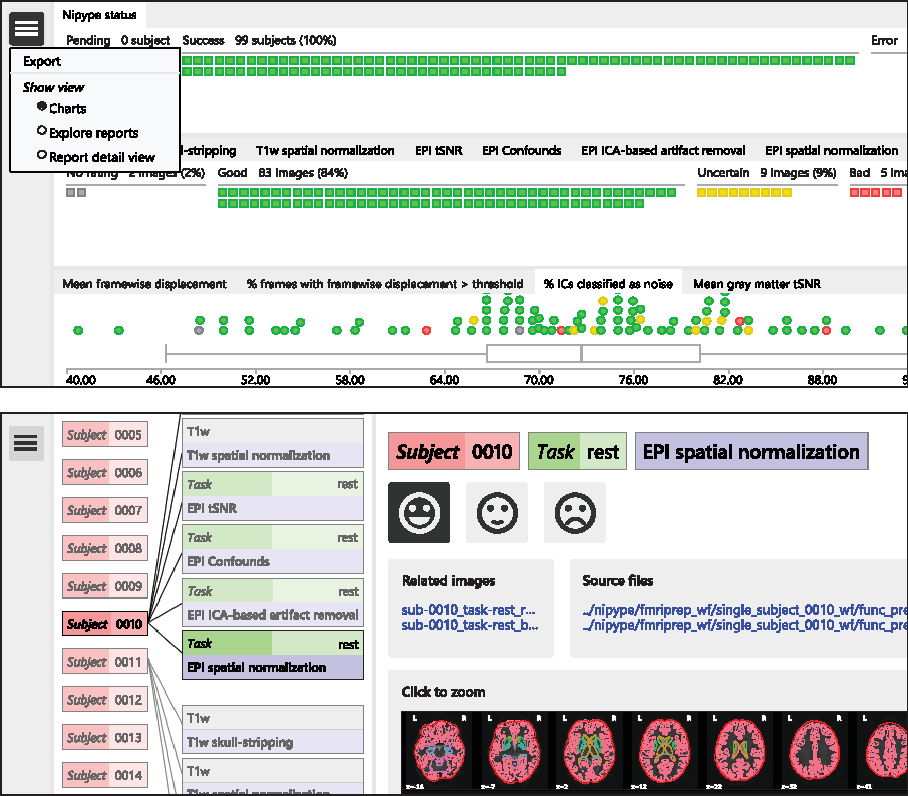
\includegraphics[width=\linewidth]{fig/quality_assessment-crop}
\caption{\textbf{Quality assessment user interface.} The top panel shows
the charts view, containing one chart for processing status, one for
quality ratings and one for image quality metrics. In the top left
corner, the navigation menu is open, which shows the option to export
ratings for use in group statistics. The bottom panel contains a 
screenshot of the explorer view that allows the user to navigate across
subjects and image types. The explorer view shows the currently selected
report image on the right, along with its rating, related images, and the
source files that were used to construct it.}\label{fig:qa}
\end{adjustwidth}
\end{figure}

\subsection{Feature extraction}\label{sec:featureextraction}

Following preprocessing, \soft{HALFpipe} can extract several
\term{features} that are commonly used in resting-state and task-based
analysis. These include various ways of examining functional connectivity
between brain regions (seed-based connectivity, network-template (or dual)
regression, atlas-based connectivity matrices), as well as measures of
local activity (ReHo, fALFF). \soft{HALFpipe} allows the user to choose
several region-of-interest masks (seeds), template networks, and atlases,
for which a threshold indicates the minimum overlap the user requires
between seeds, template networks, or atlas regions and the subjects' fMRI
data. For each feature, the user can change the default settings for
spatial smoothing and temporal filtering, and choose the confounds to be
removed. The user is offered the option to extract the same feature
multiple times, each time varying the preprocessing, confound, and
denoising settings to explore the impact of analytical decisions in a
\term{multiverse analysis}. Of note, for selected features some options are
not available. For example, spatial smoothing is disabled for atlas-based
connectivity matrices \parencite{10.1111/ejn.13717}, or performed \emph{after}
ReHo and fALFF have been calculated (see Table~\ref{table:settings}).

A brief description of the features is provided in Box~\ref{box:features}.

\subsection{Group-level statistics}

Group-level statistics on individual features can be performed with
\soft{FSL}'s FLAME algorithm. Subjects who had poor quality data in the
interactive quality assessment are excluded. In addition, subjects can be
excluded based on movement by selecting the maximum allowed mean framewise
displacement (FD) and percentage of outlier frames (i.e., frames with
motion higher than the specified FD threshold).

For group-level statistics, users can choose to calculate the intercept
only (i.e., mean across all subjects) or run flexible factorial models. For
the latter, \soft{HALFpipe} prompts the user to specify the path to a
covariates file (multiple file formats are supported) containing subject
identifiers, group membership, and other variables, and to specify whether
these are continuous or categorical. Missing values in the covariates file
can be handled with either listwise deletion or mean substitution. The user
can specify main effects and interactions between variables, while
within-group regressions against a continuous variable (e.g., symptom
severity) is also possible.

\begin{featurebox}[label={box:features}]{Overview of HALFpipe features}

\paragraph{Task-based activations}

A first-level general linear model (GLM) is run for event-related or block
designs. GLM regressors describing the stimulus presentations for each of
the task conditions are convolved with a double Gamma HRF and the overall
model is fit for each voxel in the brain using \soft{FSL FILM}
\parencite{woolrich_temporal_2001}. Contrasts of interest are tested, which
results in a whole-brain task activation map for comparisons between task
conditions.

\paragraph{Seed-based connectivity}

Average BOLD time series are extracted from a region of interest (seed),
which is defined by a binary mask image. This time series is used as a
regressor in a first-level GLM, where the model is fit for each voxel in
the brain using \soft{fsl\_glm}. This results in a whole-brain functional
connectivity map that represents the connectivity strength between the ROI
and each voxel in the brain.

\paragraph{Network-template (or dual) regression}

Subject-specific representations of connectivity networks (e.g., default
mode, salience, task-positive networks) are generated using dual regression
\parencite{beckmann_dual_reg_2009} with \soft{fsl\_glm}. In a first
regression model, the set of network template maps is regressed against the
individual fMRI data, which generates time series for each of the template
networks. Next, a second regression model is run, regressing the network
time series against the individual fMRI data. This generates
subject-specific spatial representations of each of the template networks,
which can be considered to represent the voxelwise connectivity strength
within each of the networks.

\paragraph{Atlas-based connectivity matrix}

Average time series are extracted from each region of a brain atlas of
choice using custom code inspired by \soft{Pypes}
\parencite{10.3389/fninf.2017.00025} and \soft{Nilearn}
\parencite{10.3389/fninf.2014.00014}. From these, a pairwise connectivity
matrix between atlas regions is calculated using Pearson product-moment
correlations using \soft{Pandas} \parencite{mckinney-proc-scipy-2010}, which
represent the pairwise functional connectivity between all pairs of regions
included in the atlas.

\paragraph{Regional homogeneity (ReHo)}

Local similarity (or synchronization) between the time series of a given
voxel and its nearest neighboring voxels is calculated using Kendall's
coefficient of concordance \parencite{10.1016/j.neuroimage.2003.12.030} using
\soft{FATCAT}'s \soft{3dReHo} which is distributed with \soft{AFNI}
\parencite{10.1089/brain.2013.0154}.

\paragraph{Fractional amplitude of low frequency fluctuations (fALFF)}

Variance in amplitude of low frequencies in the BOLD signal is calculated,
dividing the power in the low frequency range (0.01--0.1 Hz) by the power
in the entire frequency range \parencite{10.1016/j.jneumeth.2008.04.012} with a
customized version of the \soft{C-PAC} implementation of fALFF.\@

\end{featurebox}


\section{Discussion}

Large samples are essential for recent neuroimaging applications, such as
imaging-genetics association studies, training of complex machine learning
models, and even unsupervised learning. This demand has stimulated efforts
to pool data from multiple observational studies, which typically incur
greater bias than studies designed \emph{a priori} to address a specific
scientific question. Within ENIGMA, we developed \soft{HALFpipe} to support
harmonization of task-based and resting-state fMRI data analysis and
quality assessment across multiple labs and cohorts. \soft{HALFpipe}
bundles all software tools, library functions, and other dependencies by
containerizing the requisite components in a Singularity
\parencite{10.1371/journal.pone.0177459} and Docker (Docker Inc.) release.
Containerization ensures that all software dependencies and the runtime
environment are provided. Therefore, containerized software such as
\soft{HALFpipe} can run reliably regardless of the computing environment
where it is installed, be it a laptop, computational cluster, or cloud
computing service \parencite{10.1016/j.cels.2018.03.014}.

The design, implementation, and testing of the \soft{HALFpipe} workflow
resulted in its 1.0 version release in early 2021. Several thousand
resting-state fMRI datasets from 29 ENIGMA PTSD consortium sites have
already been analyzed as part of the first published report to employ
\soft{HALFpipe} \parencite{weis_thesis}, while analyses of other large
multi-site datasets are currently underway in several ENIGMA working
groups, including the ENIGMA task-based fMRI working group \parencite{veer_enigma_2019}. 
Running \soft{HALFpipe} requires approximately 8 to 20 GB of RAM per
computer or cluster node and 6 to 10 hours to complete on a single
processor core. The exact resource usage depends on voxel resolution and
the number of volumes in the fMRI data. The number of features the user
chooses has a negligible impact on processing time.

The \soft{HALFpipe} user experience includes an interactive user interface
to facilitate rapid analysis prototyping while preserving the ability to
script automated analyses of large datasets via configuration files in JSON
format with detailed prescriptions of the dataset, analyses steps, and
input parameters. Importantly, \soft{HALFpipe} accommodates concurrent
harmonized processing of task-based and resting-state fMRI data, which
facilitates cross-modal comparisons between the two fMRI modalities.

Our implementation of \soft{HALFpipe} enables users to tackle consortium
analyses of multi-cohort fMRI data with highly uniform application of
methods. Specifically, we have established a standardized process and
analysis methodology that involves a pre-specified: (1) ensemble of
software tools, (2) software version for each tool, (3) set of user-defined
parameters, (4) analytic steps, (5) sequence of analytic steps, (6) quality
assessment process, and (7) criteria for excluding substandard data. Thus,
\soft{HALFpipe} promotes the seamless implementation of a standardized
process (preprocessing and feature extraction) at each site and/or cohort
prior to initiating group level statistics. Such capabilities hold the
promise of significantly advancing basic neuroscience, and particularly
clinical neuroscience, by supporting the execution of multi-site
multi-cohort studies of several hundred or several thousand samples ---
ultimately supporting harmonized cross-disorder comparisons. While not part
of the \soft{HALFpipe} workflow, cross-site/platform harmonization
techniques for neuroimaging have recently experienced a dramatic increase
\parencite{pezoulas2020medical,10.1016/j.neuroimage.2017.11.024,10.1016/j.media.2020.101879}.
Much of this methodological innovation has arrived on the heels of earlier
developments in cross-platform harmonization of genetic data
\parencite{10.1186/s12859-019-2641-8,10.1093/biostatistics/kxj037,10.1093/bioinformatics/btx147,10.1038/nbt.4091}.
These advances in harmonization of neuroimaging data are expected to
manifest synergy with standardized workflows such as \soft{HALFpipe}, as
both elements are essential to large-scale imaging consortium efforts
\parencite{thompson_enigma_2020}.

The implementation of quality metrics for fMRI data has been an incremental
process that has moved steadily towards establishing empirically-informed
best practices. Historically, quality criteria have been applied unevenly
across research labs. Recent years have witnessed a heightened awareness
about the essential role of applying systematic and principled quality
metrics to minimize confounds, for example motion artifacts
\parencite{10.1016/j.neuroimage.2011.10.018,10.1016/j.neuroimage.2013.08.048,10.1016/j.neuroimage.2013.04.001},
and widespread fMRI signal deflections
\parencite{10.1016/j.neuroimage.2020.116614}. Automated quality control methods
are being developed and adopted with increasing interest, such as the MRI
Quality Control software \soft{MRIQC} \parencite{10.1371/journal.pone.0184661}.
\soft{HALFpipe} has adopted parts of the functionality of \soft{MRIQC} with
an enhanced user experience that generates quality reports via a
web-browser-based interface to facilitate rapid viewing, screening, and
selection of individual subject data for inclusion or exclusion. The
application of uniform quality assessment procedures is particularly
important when mega-analyzing and even meta-analyzing multi-site/scanner
data, as is done in ENIGMA.\@ That is, study variables that segregate by site
are more likely to lead to confounds without the uniform implementation of
quality assessment across sites
\parencite[e.g.][]{10.1016/j.media.2020.101879}. With its harmonized quality
procedures, \soft{HALFpipe} aims to minimize such effects.

\subsection{Limitations}

Computing platforms that are likely to differ between sites are known to
introduce subtle differences in output attributable to operating systems
and hardware \parencite{10.1371/journal.pone.0038234}. Collecting raw
multi-site data at one central site prior to \soft{HALFpipe} processing
ensures that the same computing platform can be used to process all data.
While optimal, this is often not practical due to restrictions on data
sharing, even when the data is completely de-identified (i.e., when linking
data to protected health or other sensitive information is no longer
possible).

\soft{HALFpipe} offers harmonization through uniform processing of fMRI
data, but other sources of non-uniformity are beyond its scope. Recent
advances in cross-site/platform harmonization may additionally correct for
differences in site, scanner hardware, or computation on different
processors
\parencite{pezoulas2020medical,10.1016/j.neuroimage.2017.11.024,10.1016/j.media.2020.101879}.
Such methods could be applied to extracted \soft{HALFpipe} features, either
centralized or through distributed computation using tools such as
\soft{COINSTAC} \parencite{plis_coinstac_2016}, to yield results that are
potentially more generalizable.

\subsection{Conclusion}

\soft{HALFpipe} provides a standardized workflow that encompases the
essential elements of task-based and resting-state fMRI analyses, builds on
the progress and contributions of \soft{fMRIPrep} developers, and extends
capabilities beyond preprocessing steps with a diverse set of
post-processing functions. \soft{HALFpipe} represents a major step toward
addressing the reproducibility crisis in functional neuroimaging by
offering a workflow that maintains details of user options, steps performed
in analyses, metadata associated with analyses, code transparency,
containerized installation, and the ability to recreate the runtime
environment, while implementing empirically-supported best-practices
adopted by the functional neuroimaging community.


\section{Acknowledgements}

This work has been supported by a Grant from the German Research
Foundation to S.E. and H.W. (DFG ER 724/4--1, WA 1539/11--1).
P.M.T. received research grant funding from Biogen, Inc., for research
unrelated to this manuscript.
L.S. received funding from the National Institutes of Health (NIH RO1
MH117601 and NHMRC Career Development Fellowship 1140764).
R.A.M received funding from National Institutes of Health (NIH R01
MH111671).
I.V. received funding from the European Union's Horizon 2020 research
and innovation programme under under Grant Agreement number 777084
(DynaMORE project).

\printbibliography

\end{document}
